%%%%%%%%%%%%%%%%%%%%%%%%%%%%%%%%%%%%%%%%%%%%%%%%%%%%%%%%%%%%%%%%%%%%%%%%
% Plantilla TFG/TFM
% Universidad de A Coruña. Facultad de Informática
% Realizado por: Welton Vieira dos Santos
% Modificado: Welton Vieira dos Santos
% Contacto: welton.dossantos@udc.es
%%%%%%%%%%%%%%%%%%%%%%%%%%%%%%%%%%%%%%%%%%%%%%%%%%%%%%%%%%%%%%%%%%%%%%%%


\chapter{Modelo de Comunicación}

\section{Plan de comunicación}
En este caso, la comunicación que se realiza es simplemente entre nuestro sistema y otros agentes para obtener dados referentes al mercado.

\subsection{Diagrama de diálogo}

  \begin{figure}[H]
    \centering
    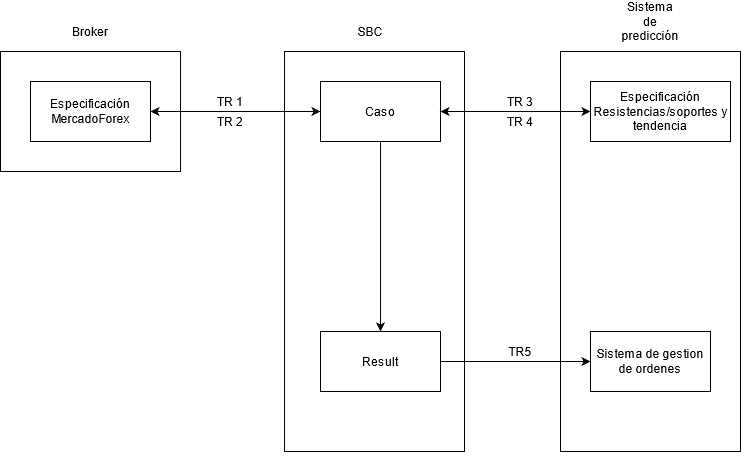
\includegraphics[scale=0.50]{imagenes/Comunicaciones.png}
    \caption{\label{fig:Comunicaciones}Diagrama de dialogo}
  \end{figure}
  
\subsection{Descripción de las transacciones}

\begin{table}[H]
  \scriptsize
  \begin{tabularx}{\textwidth}{|l|X|} \hline
    & \textbf{Formulario CM-1: Especificación de transacciones - TR1} \\
    \hline\hline
    {Nombre de la transacción} & Solicitar datos iniciales\\
    \hline  
    \textsc{Objecto de informacion} & \textsc{El SBC solicita la especificacion del Mercado Forex al Broker}\\ 
    \hline
    \textsc{Agentes involucrados} & \textsc{Emisor: SBC, Receptor: Broker}\\ 
    \hline
    \textsc{Plan de comunicación} & \textsc{Especificado en las Figura \ref{fig:Comunicaciones} }\\ 
    \hline
    \textsc{Restricciones} & \textsc{El Broker debe estar listo para su uso}\\ 
    \hline
    \textsc{Especificación del intercambio} & \textsc{Tipo ASK}\\ 
    \hline
  \end{tabularx}
  \caption{\label{tab:TR1}Formulario CM-1 para TR-1}
\end{table}
  

\begin{table}[H]
  \scriptsize
  \begin{tabularx}{\textwidth}{|l|X|} \hline
    & \textbf{Formulario CM-1: Especificación de transacciones - TR2} \\
    \hline\hline
    {Nombre de la transacción} & Recibir datos iniciales\\
    \hline  
    \textsc{Objecto de informacion} & \textsc{El broker envía la especificacion del Mercado Forex al SBC}\\ 
    \hline
    \textsc{Agentes involucrados} & \textsc{Emisor: Broker, Receptor: SBC}\\ 
    \hline
    \textsc{Plan de comunicación} & \textsc{Especificado en la Figura \ref{fig:Comunicaciones} }\\ 
    \hline
    \textsc{Restricciones} & \textsc{El SBC debe estar listo para su uso}\\ 
    \hline
    \textsc{Especificación del intercambio} & \textsc{Tipo REPLY}\\ 
    \hline
  \end{tabularx}
  \caption{\label{tab:TR2}Formulario CM-1 para TR-2}
\end{table}


\begin{table}[H]
  \scriptsize
  \begin{tabularx}{\textwidth}{|l|X|} \hline
    & \textbf{Formulario CM-1: Especificación de transacciones - TR3} \\
    \hline\hline
    {Nombre de la transacción} & Solicitud de la Especificación de Resistencias, Soportes y Tendencia\\
    \hline  
    \textsc{Objecto de informacion} & \textsc{El SBC solicita la especificacion de resistencias, soportes y tendencia al Sistema de Predicción}\\ 
    \hline
    \textsc{Agentes involucrados} & \textsc{Emisor: SBC, Receptor: Sistema de predicción.}\\ 
    \hline
    \textsc{Plan de comunicación} & \textsc{Especificado en la Figura \ref{fig:Comunicaciones} }\\ 
    \hline
    \textsc{Restricciones} & \textsc{La especificacion del MercadoForex debe estar disponible y El Broker debe estar listo para su uso}\\ 
    \hline
    \textsc{Especificación del intercambio} & \textsc{Tipo ASK}\\ 
    \hline
  \end{tabularx}
    \caption{\label{tab:TR3}Formulario CM-1 para TR-3}
\end{table}

\begin{table}[H]
  \scriptsize
  \begin{tabularx}{\textwidth}{|l|X|} \hline
    & \textbf{Formulario CM-1: Especificación de transacciones - TR4} \\
    \hline\hline
    {Nombre de la transacción} & Recepción de las Especificaciónes de Resistencias, Soportes y Tendencia\\
    \hline  
    \textsc{Objecto de informacion} & \textsc{El sistema de predicción envia las especificaciones de resistencias , soportes y tendencia al SBC}\\ 
    \hline
    \textsc{Agentes involucrados} & \textsc{Emisor: Sistema de predicción. Receptor: SBC}\\ 
    \hline
    \textsc{Plan de comunicación} & \textsc{Especificado en la Figura \ref{fig:Comunicaciones}}\\ 
    \hline
    \textsc{Restricciones} & \textsc{La especificacion del MercadoForex debe estar disponible y el SBC debe estar listo para su uso}\\ 
    \hline
    \textsc{Especificación del intercambio} & \textsc{Tipo REPLY}\\ 
    \hline
  \end{tabularx}
    \caption{\label{tab:TR4}Formulario CM-1 para TR-4}
\end{table}

\begin{table}[H]
  \scriptsize
  \begin{tabularx}{\textwidth}{|l|X|} \hline
    & \textbf{Formulario CM-1: Especificación de transacciones - TR5} \\
    \hline\hline
    {Nombre de la transacción} & Reporte de resultados\\
    \hline  
    \textsc{Objecto de informacion} & \textsc{El SBC envia una solucion del caso al Sistema de predicción}\\ 
    \hline
    \textsc{Agentes involucrados} & \textsc{Emisor: SBC, Receptor: Sistema de prediccion}\\ 
    \hline
    \textsc{Plan de comunicación} & \textsc{Especificado en la Figura \ref{fig:Comunicaciones}}\\ 
    \hline
    \textsc{Restricciones} & \textsc{Es necesario que el SBC y el Sistema de prediccion esten sincronizados}\\ 
    \hline
    \textsc{Especificación del intercambio} & \textsc{Tipo REPORT}\\ 
    \hline
  \end{tabularx}
    \caption{\label{tab:OM1}Formulario CM-1 para TR-5}
\end{table}


